%\begin{frame}
  %\frametitle{Motivation}
  % a comment
%  \begin{figure}[htbp!]
%    \begin{center}
%      
\includegraphics[height=4cm]{./images/kitten}
%    \end{center}
%          \caption{A caption describing the image. \cite{lastname_firstword_1900}.}
%    \label{fig:kittenfigure}
%  \end{figure}
%\end{frame}

\begin{frame}
  \frametitle{Motivation}
   \begin{itemize}
   
   \item Dynamic transition analysis to minimize CO$_2$ emissions in Japan.
   
   \item Focus on optimizing \textbf{electricity supply}.
   
   \item \textbf{I$^2$CNER goal:} Reduce emissions by 80\% from 1990 levels by 2050, 
   
   \item After 2050: emissions held constant until 2100 if possible.
   
   \item Energy supply includes conventional and some I$^2$CNER technology.
   
   \item Using The Integrated MARKAL-EFOM System (TIMES).
   \end{itemize}
%        Frames (slides) can have ``blocks.'' 
%        \begin{block}{This one is about a cat}
%                A cat in a hat.
%        \end{block}
%        \begin{block}{A cat}
%                In a hat.
%
%                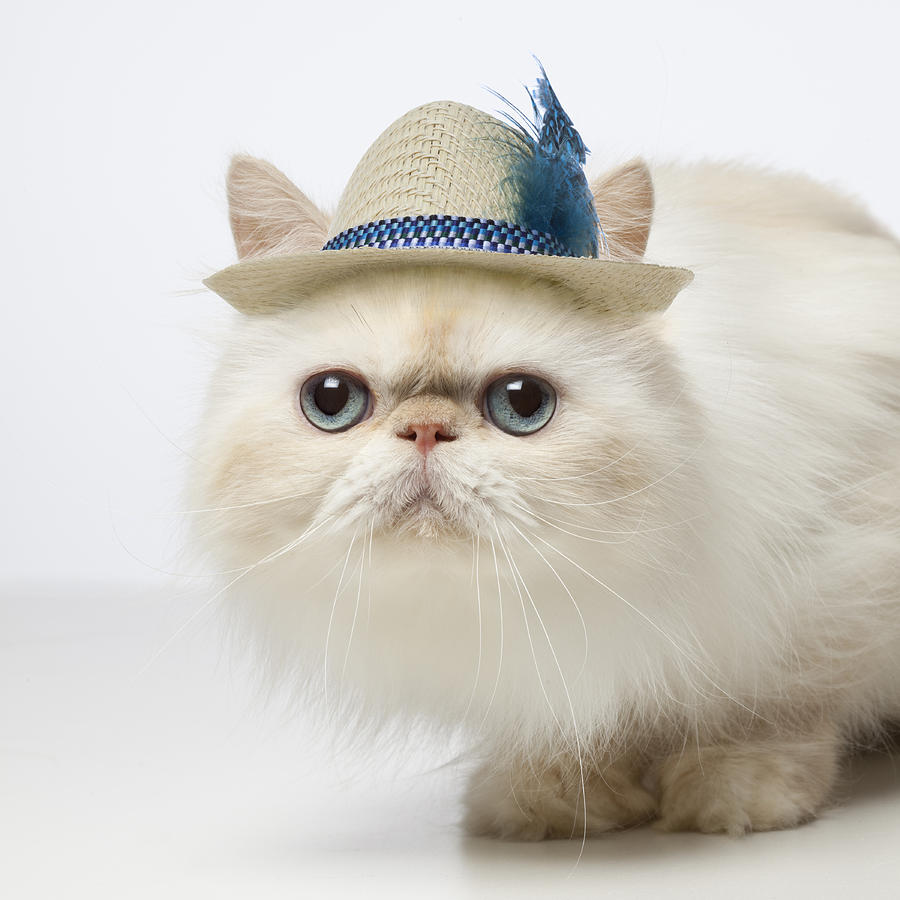
\includegraphics[height=0.2\textheight]{./images/catinhat}
%        \end{block}
        
\end{frame}
